%!TeX program = xelatex
\documentclass[12pt,hyperref,a4paper,UTF8,AutoFakeBold,AutoFakeSlant]{ctexart}
\usepackage{zjureport}
\graphicspath{ {./figures/} } % where to find figures

%%-------------------------------正文开始---------------------------%%
\begin{document}

%%-----------------------封面--------------------%%
% \cover
% \thispagestyle{empty} % 首页不显示页码

%%------------------摘要-------------%%
% \clearpage
% \begin{abstract}
% \normalsize
% The abstract

% \end{abstract}

% \thispagestyle{empty} % 首页不显示页码

%%--------------------------目录页------------------------%%
% \clearpage
% \tableofcontents

% \thispagestyle{empty} % 首页不显示页码

%%------------------------正文页从这里开始-------------------%
\clearpage
\pagenumbering{arabic}
\linespread{1.5}

%%可选择这里也放一个标题
%\begin{center}
%    \title{ \Huge \textbf{{标题}}}
%\end{center}



\section{问题要求}
\par 结合生活中案例,利用物体检测类神经网络(如YOLO系列),实现物体的检测和识别。
\begin{itemize}[nosep]
    \item 要求1:类别数量不得低于4个;
    \item 要求2:每个类别的样本图片数量不得多于20个。
\end{itemize}

形成一个专题报告,详细描述选择该网络的理由、数据来源、训练环境、训练过程、验证和测试情况。

\section{实现和说明}

\subsection{技术路线}
\subsubsection{网络构架}
针对物体检测,我们备选的构架是CNN和Transformer。两种构架的备选模型分别是YOLO\cite{YOLO}系列和Paligemma\cite{PaliGemma}。
针对问题和网络特性,最终选择YOLO,理由如下:
\begin{itemize}[nosep]
    \item \textbf{数据量极小}:根据要求,每个类别仅20最多张图片。ViT论文\cite{ViT}指出,由于CNN带有归纳偏置,相比起Transformers,小数据集下CNN很有可能表现更好。此外,对于每类仅20张图片的训练集大小,无法有效微调3B参数的Paligemma模型;相比之下,训练一个数据量10M左右的CNN更为可行。
    \item \textbf{资源受限}:我们使用RTX 4060 8GB RAM显卡,而Paligemma微调需要12GB显存才可能微调全部Attnetion Layers。尽管通过LoRA或者QLoRA,可能通过较为有限的资源对Transformer模型进行微调,但是能够对模型产生的影响也相对应地更小。相比之下,YOLOv8更加轻量适配,完全可以对全部权重进行快速有效的微调。
\end{itemize}

\subsubsection{YOLO具体路线}
具体方案选择:
\begin{itemize}[nosep]
    \item \textbf{YOLOv8s(small)}:11.2M参数,适合细粒度分类且不易过拟合,适配已有资源的8GB显存,训练快,对于较少种类的进行视觉检测已经足够。
    \item \textbf{迁移学习}:在进行模型fine-tuning和从头训练两个路线之间,我们选择使用前者,使用基于COCO数据集预训练的模型进行权重微调。这是因为预训练的模型的较前的神经网络层数已经学习到了一些有效的patterns,而使用80张图片从头训练一个较大的模型可能导致效果不佳。
    \item \textbf{强数据增强}:实验允许的训练数据极小,为了进行有效的学习,大量使用复制粘贴、旋转缩放、颜色变换等方法进行数据增强,以补偿数据不足。
\end{itemize}

\subsection{任务和数据}

\textbf{任务设定:} 为了充分验证YOLO在少样本学习(few-shot learning)场景下的能力,我们选择了比较具有挑战性的任务,对猫的品种进行目标识别和检测。与猫狗分类等粗粒度任务不同,不同猫品种之间的视觉差异相对更小,需要模型学习更加精细和有效的特征表示以进行分类。

\textbf{数据来源:} 使用Cat-Breeds-Detection-Dataset\footnote{https://github.com/AWREDD/Cat-Breeds-Detection-Dataset},该数据集已按YOLO格式组织,包含标注完整的边界框信息,边界框标注了猫的头部。原始数据集涵盖5个猫品种,每个品种包含约300张图片。

\textbf{数据集构建:} 为满足实验要求(每类不多于20张训练图片),我们挑选了4个较有视觉区分度的品种:
\begin{itemize}[nosep]
    \item {波斯猫(Persian):} 长毛,扁脸特征明显
    \item {斯芬克斯猫/加拿大无毛猫(Sphynx):} 无毛品种,皮肤褶皱特殊
    \item {布偶猫(Ragdoll):} 长毛,面部色块分布较为明显
    \item {苏格兰折耳猫(Scottish Fold):} 深色较多,有独特的折耳特征
\end{itemize}

其中,波斯猫和布偶猫由于都具有长毛特征,较容易混淆;无毛猫特征明显,容易分辨。在构建数据集时,每个品种选取20张训练图片和5张验证图片。样本展示如图\ref{fig:dataset}。

\begin{figure}[H]
    \centering
    \includegraphics[width=0.8\textwidth]{dataset_visualization.png}
    \caption{数据集样本展示}
    \label{fig:dataset}
\end{figure}

\subsection{训练环境}

实验在以下硬件和软件环境中进行:

\begin{itemize}[nosep]
    \item {GPU:} NVIDIA RTX 4060(8GB显存,约7GB可用)
    \item {CPU:} Intel Core i7-14650HX
    \item {内存:} 24GB
    \item {操作系统:} Ubuntu 20.04 LTS
    \item {Python版本:} 3.8
\end{itemize}

关键Python包详见附录表\ref{tab:packages}。训练超参数配置详见附录表\ref{tab:training_args},其中包含数据增强强度、优化器设置等信息。

\subsection{训练过程}

\textbf{迁移学习:} 训练采用在COCO数据集上预训练的YOLOv8s模型作为起点。由于COCO数据集中不包含猫的具体品种标注,预训练模型仅能识别``猫''这一通用类别(见图\ref{fig:pretrained})。通过微调,模型可以学习到区分不同品种的细节特征,实现特殊领域的物体识别。

\begin{figure}[H]
    \centering
    \includegraphics[width=0.8\textwidth]{pretrained_test_result.png}
    \caption{预训练模型检测效果}
    \label{fig:pretrained}
\end{figure}

\textbf{数据增强:} 针对仅80张训练图片的数据稀缺问题,我们使用了大量地数据增强。图\ref{fig:aug}展示了经马赛克、颜色抖动、旋转缩放等增强后的效果。每张图片在每个epoch都经历不同的随机变换,有效扩充数据多样性,提高了模型的泛化能力,避免了模型过拟合。

\begin{figure}[H]
    \centering
    \includegraphics[width=0.9\textwidth]{train_batch2.jpg}
    \caption{训练数据增强效果}
    \label{fig:aug}
\end{figure}

\textbf{训练过程和指标:} 训练中,loss呈较为稳定下降的趋势(见图\ref{fig:metrics})。分类loss和标注框loss同时下降,说明模型在品种分类和定位能力上都有提升。尽管设置150轮训练,Early Stopping机制在43轮时触发,表明模型已充分收敛。最终验证集准确率和召回率均达60\%以上,mAP50和mAP50-95指标也有所上升,表明了训练的有效性。

\begin{figure}[H]
    \centering
    \includegraphics[width=1.0\textwidth]{results.png}
    \caption{训练和表现指标变化曲线}
    \label{fig:metrics}
\end{figure}

\subsection{验证和测试}
除去使用图\ref{fig:metrics}中的指标进行训练结果的验证,我们还对训练结果进行了可视化。图\ref{fig:comparison1}, \ref{fig:comparison2}展示了预训练模型和微调后模型在同一张验证图片上的检测效果对比。可以明显看出,微调后的模型能够更有效地识别出具体的猫品种,而预训练模型只能标注通用的``cat''类别。在图\ref{fig:comparison1}中,微调后的模型正确辨认出了所有猫的品种,而微调前的模型甚至将无毛猫辨认为``dog''。然而,在小样本上学习的模型仍然可能出现错误。在图\ref{fig:comparison2}中,微调后的模型错误地将波斯猫辨认为布偶猫。

\begin{figure}[H]
    \centering
    \includegraphics[width=1.0\textwidth]{model_comparison_2.png}
    \caption{模型对比结果1}
    \label{fig:comparison1}
\end{figure}

\begin{figure}[H]
    \centering
    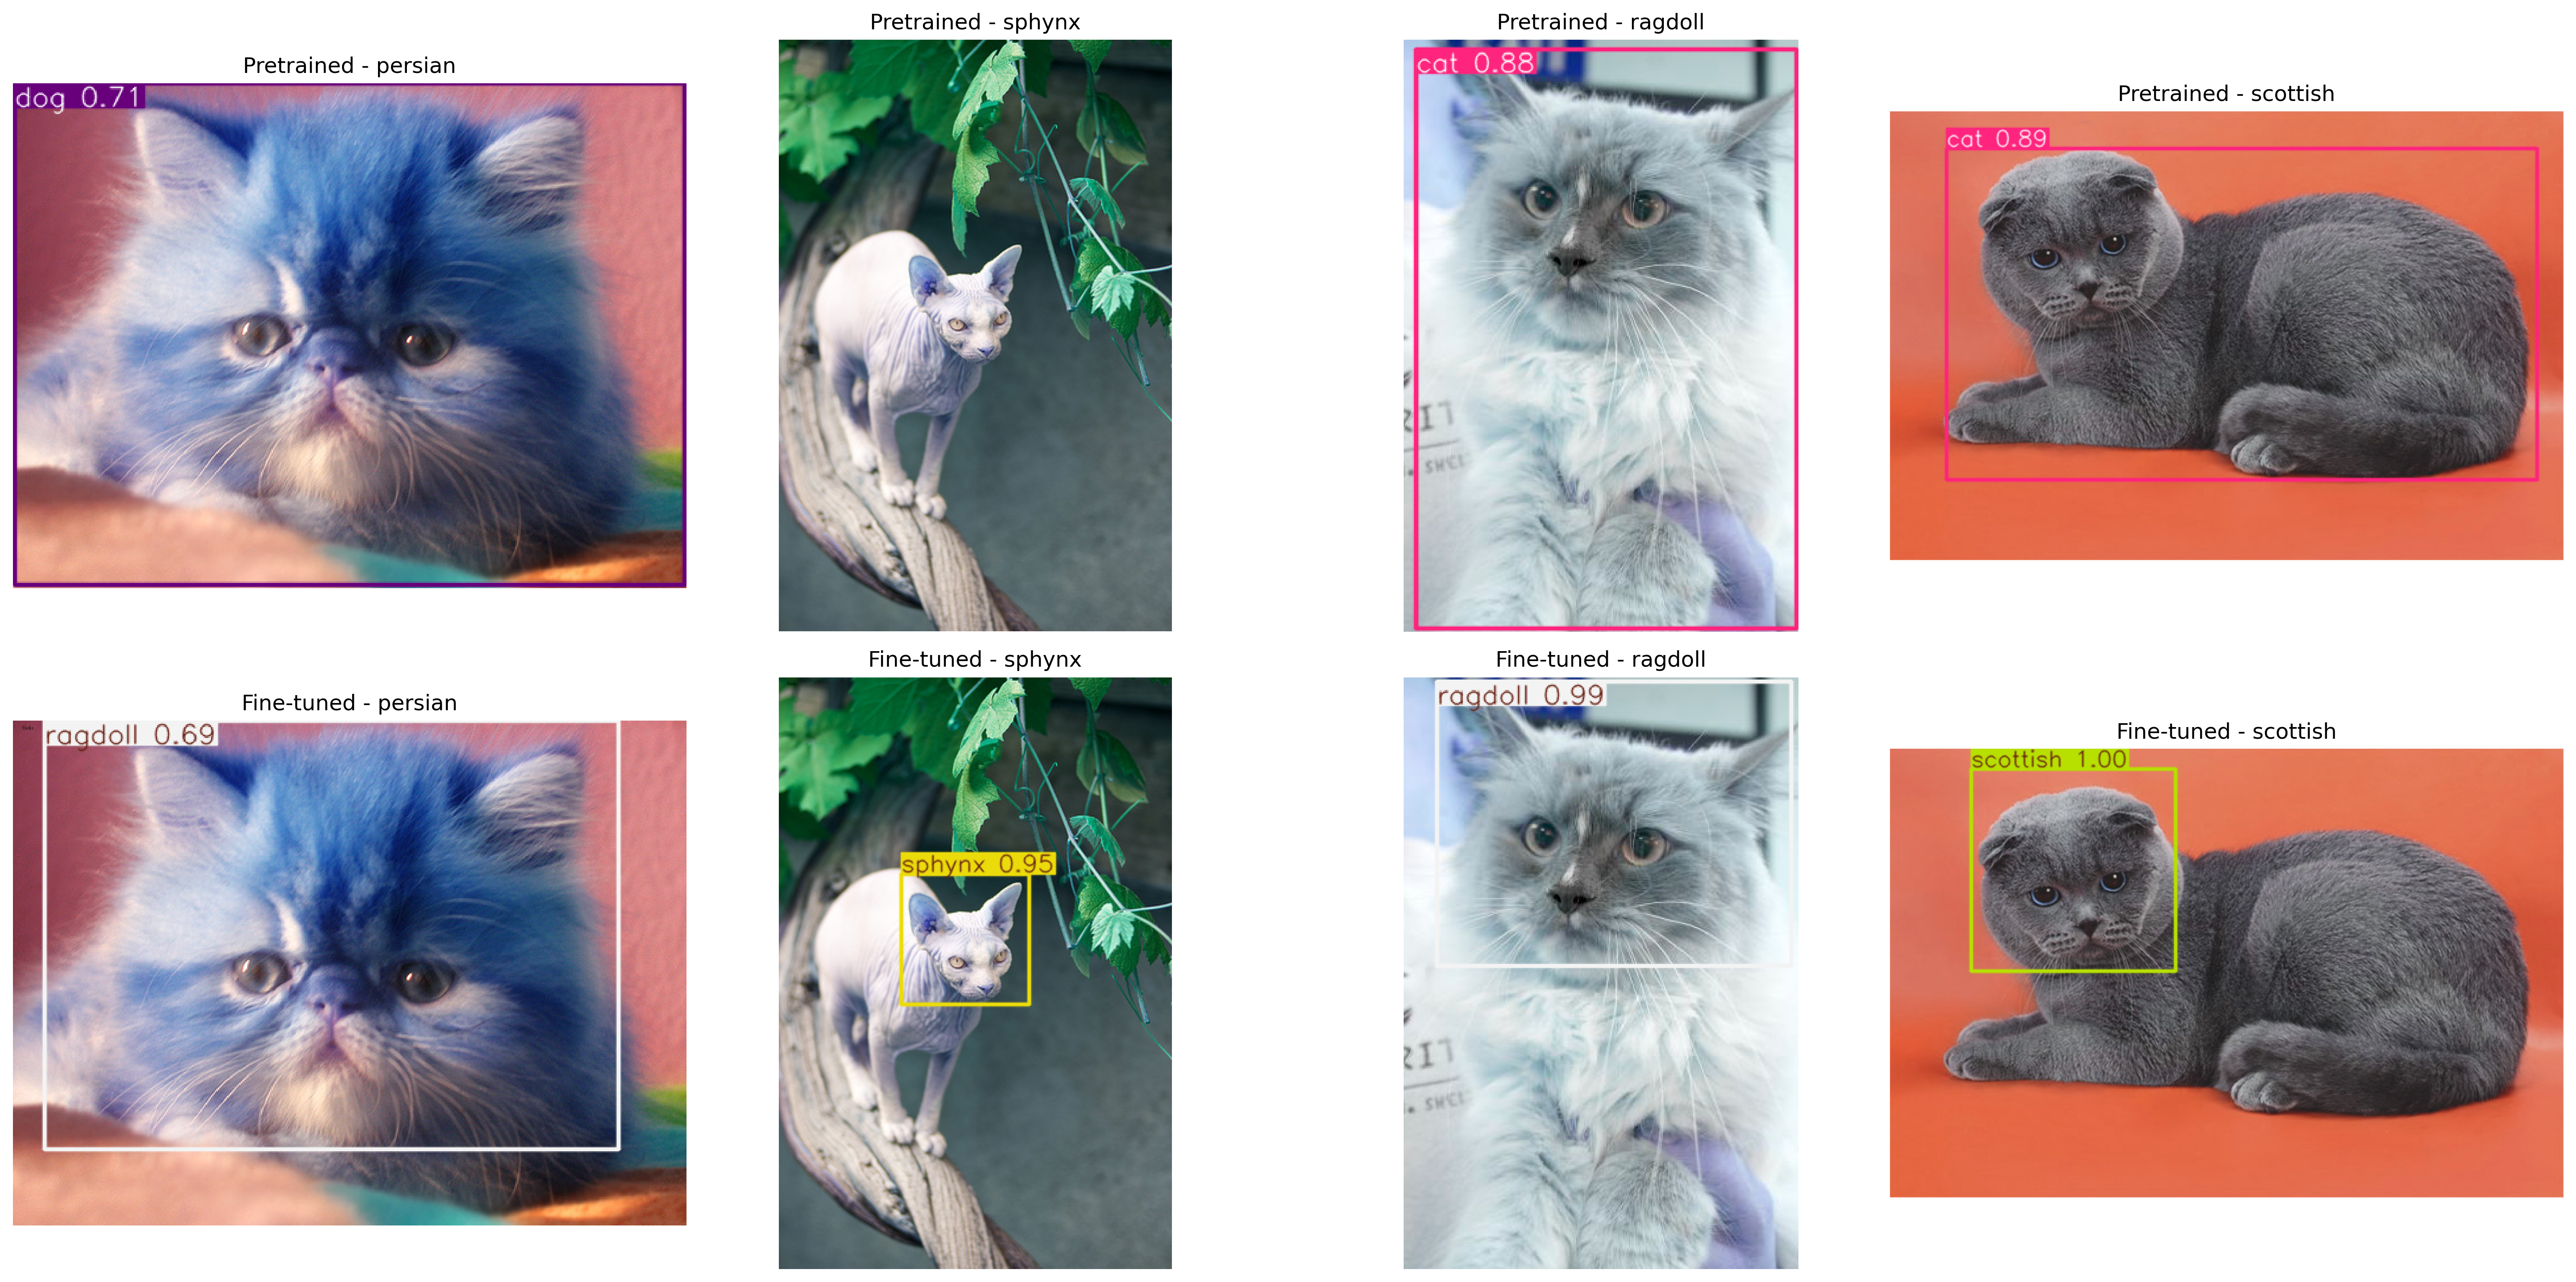
\includegraphics[width=1.0\textwidth]{model_comparison.png}
    \caption{模型对比结果2}
    \label{fig:comparison2}
\end{figure}

总体而言,针对猫的品种辨认,微调后的模型有效地学习到了猫的品种特征,也习得了对应品种猫面部位置的知识。如果训练样本量增加,微调结果将更加有效。

\subsection*{附录}

\begin{table}[H]
    \centering
    \caption{关键Python包版本信息}
    \label{tab:packages}
    \begin{tabular}{ll}
        \hline
        \textbf{包名称} & \textbf{版本} \\
        \hline
        torch & 2.4.1+cu124 \\
        torchvision & 0.19.1+cu124 \\
        ultralytics & 8.3.43 \\
        opencv-python & 4.10.0 \\
        numpy & 1.24.1 \\
        matplotlib & 3.7.2 \\
        pandas & 2.0.3 \\
        PyYAML & 6.0.2 \\
        tqdm & 4.66.5 \\
        \hline
    \end{tabular}
\end{table}

\begin{table}[H]
    \centering
    \caption{训练超参数配置}
    \label{tab:training_args}
    \begin{tabular}{ll}
        \hline
        \textbf{参数} & \textbf{数值} \\
        \hline
        epochs & 150 \\
        batch size & 32 \\
        image size & 640 \\
        optimizer & AdamW \\
        learning rate & 0.001 \\
        weight decay & 0.0005 \\
        saturation augmentation & 0.7 \\
        value augmentation & 0.4 \\
        rotation range & 15.0° \\
        scale range & 0.5 \\
        mosaic probability & 1.0 \\
        mixup probability & 0.2 \\
        copy-paste probability & 0.3 \\
        \hline
    \end{tabular}
\end{table}

\reference

\end{document}